%% Seminar deck: Closer to New York than to Frankfurt? (working paper, 2026)
%% 14 slides, yieldcartography house theme, academic-seminar register.
%% Built from the SSRN working paper (regime-and-power framing). No venue
%% disclosed.
\documentclass[aspectratio=169,11pt]{beamer}
\usepackage{beamerthemeyc}
\renewcommand{\deckfootertitle}{Dec (2026) · Closer to New York than to Frankfurt? · SSRN 6695444}

\begin{document}

% 1 ---------------------------------------------------------------------------
\begin{frame}[plain]
  \vspace{2mm}
  {\ttfamily\scriptsize\color{ycmuted}SEMINAR DECK · YIELDCARTOGRAPHY.COM}\\[-0.3em]
  {\color{ycrule}\rule{\textwidth}{0.5pt}}
  \vspace{4mm}

  {\fontsize{19}{23}\selectfont\bfseries\color{ycink}Closer to New York than to Frankfurt?\par}
  \vspace{2mm}
  {\normalsize\color{ycmuted}The expectations hypothesis in Poland, the US and the euro area.\par}
  \vspace{6mm}
  {\small\bfseries Marcin Dec\par}
  {\footnotesize\color{ycmuted}Kozminski University \& FAME|GRAPE, Warsaw\par}
  \vspace{3mm}
  {\ttfamily\scriptsize\color{ycaccent}Working paper · SSRN 6695444 · doi:10.2139/ssrn.6695444 · under peer review\par}
  \vfill
  \raisebox{-1mm}{
\includegraphics[height=6mm]{kozminski_logo.png}}\hspace{5mm}
  \raisebox{-1mm}{
\includegraphics[height=6mm]{grape_logo.png}}\hspace{5mm}
  \raisebox{-1mm}{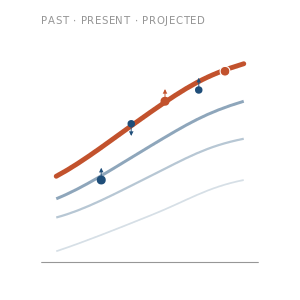
\includegraphics[height=6mm]{yc_logo.png}}
  \hfill{\ttfamily\scriptsize\color{ycmuted}NCN Preludium UMO-2020/37/N/HS4/02202}
\end{frame}

% 2 ---------------------------------------------------------------------------
\begin{frame}{Motivation}
  \kicker{The question}
  \begin{itemize}
    \item Under the pure expectations hypothesis (PEH), long yields average
          expected future short rates plus a constant premium. Its sharpest
          implementation is the Fama--Bliss type-1 regression of future yield
          changes on the scaled forward-spot spread: the null is slope
          $\beta=1$, intercept zero.
    \item Four decades of US evidence reject PEH on the FB1 grid, with
          $\beta$ estimates drifting toward and past zero. The euro-area AAA
          panel is the other natural benchmark.
    \item The question: does a less-liquid sovereign curve, here Poland,
          behave like either benchmark, and \alert{what do cross-market
          differences in rejection actually identify}: curve structure, or
          regime exposure and test power?
  \end{itemize}
\end{frame}

% 3 ---------------------------------------------------------------------------
\begin{frame}{Data and test design}
  \kicker{Three panels, five families, two inference methods}
  \small
  \begin{itemize}
    \item \textbf{Panels.} 256 monthly observations, 2005:01--2026:04. Poland:
          LW-NSS-fitted zero curves on the BondSpot panel. US: GSW zero-coupon
          panel. Euro area: ECB AAA spot-rate curve.
    \item \textbf{Test families.} Fama--Bliss type-1 (yield change) and type-2
          (holding-period return), Cochrane--Piazzesi single-factor,
          Thornton conventional and contrarian: 90 $(h,n)$ cells per market on
          the FB grid, 9 horizons $\times$ 10 maturities.
    \item \textbf{Inference.} Newey--West HAC (bandwidth $=h$) against a wild
          block bootstrap, run cell by cell. The comparison of the two is
          itself an object of interest (Bauer--Hamilton 2018).
  \end{itemize}
\end{frame}

% 3a --------------------------------------------------------------------------
\begin{frame}{The workhorse regressions}
  \kicker{Estimating equations and nulls}
  \small Fama--Bliss type-1, per horizon $h$ and maturity $n$ (months):
  \[ y^{(n-h)}_{t+h} - y^{(n)}_t \;=\; \alpha_{h,n}
     + \beta_{h,n}\,\frac{h}{\,n-h\,}\left(f^{(n-h,\,n)}_t - y^{(n)}_t\right)
     + \varepsilon_{t+h},
     \qquad H_0\!:\ \beta_{h,n}=1,\ \alpha_{h,n}=0 \]
  Cochrane--Piazzesi single factor, average excess return on the restricted
  forward-rate combination:
  \[ \overline{rx}_{t+12} \;=\; b\,\big(\hat\gamma' f_t\big) + \eta_{t+12} \]
  \begin{itemize}
    \item Overlap of $h$-period returns induces MA($h{-}1$) errors; inference
          is Newey--West with bandwidth $h$ and, in parallel, a wild block
          bootstrap that resamples residuals under the null with per-cell
          fixed seeds.
  \end{itemize}
\end{frame}

% 4 ---------------------------------------------------------------------------
\begin{frame}{Headline: PEH rejections across markets and inference methods}
  \kicker{Rejections at 5\%, by test family}
  \begin{center}
  \small
  \begin{tabular}{lcccccc}
    & \multicolumn{2}{c}{\textbf{PL}} & \multicolumn{2}{c}{\textbf{US}} & \multicolumn{2}{c}{\textbf{EA}}\\
    Test family & NW & boot & NW & boot & NW & boot\\
    \hline
    FB1 (yield change)      & 0/30 & 0/30 & 2/30 & 0/30 & \textcolor{ycsalmon}{\textbf{30/30}} & 2/30\\
    FB2 (holding period)    & 0/30 & 0/30 & 2/30 & 0/30 & 20/30 & 1/30\\
    CP (single factor)      & 0/4  & 0/4  & 1/4  & 0/4  & 4/4   & 0/4\\
    Thornton (contrarian)   & 0/26 & 0/26 & 1/26 & 0/26 & 21/26 & 1/26\\
    \hline
    \textbf{Total}          & \textbf{0/90} & \textbf{0/90} & \textbf{6/90} & \textbf{0/90}
                            & \textcolor{ycsalmon}{\textbf{75/90}} & \textbf{4/90}\\
  \end{tabular}
  \end{center}
  \vspace{2mm}
  \footnotesize\color{ycmuted} Poland never rejects under either method; the US
  rejects sparsely under NW and not at all under bootstrap; the euro area
  rejects on 75 of 90 cells asymptotically and on 4 under the bootstrap.
\end{frame}

% 5 ---------------------------------------------------------------------------
\begin{frame}{FB1 slopes at $h=12$ months: three distinct configurations}
  \kicker{Point estimates by maturity}
  \begin{center}
  \begin{tikzpicture}[x=2.6cm,y=0.72cm]
    % axes and reference lines
    \draw[ycmuted,line width=0.5pt] (0.35,-1.3) -- (0.35,2.2);
    \draw[ycrule,line width=0.4pt] (0.35,0) -- (4.55,0);
    \draw[ycrule,dash pattern=on 2pt off 2pt,line width=0.7pt] (0.35,1) -- (4.55,1);
    \node[right,font=\tiny\itshape,text=ycmuted] at (4.55,1) {PEH: $\beta=1$};
    \node[left=2pt,font=\scriptsize,text=ycmuted] at (0.35,0) {0};
    \node[left=2pt,font=\scriptsize,text=ycmuted] at (0.35,1) {1};
    \node[left=2pt,font=\scriptsize,text=ycmuted] at (0.35,2) {2};
    % groups: n=2y..5y; bars PL (salmon), US (grey-blue), EA (navy)
    \foreach [count=\g] \n/\pl/\us/\ea in {2y/-0.84/0.32/1.03, 3y/-0.97/0.59/1.29,
                                           4y/-0.99/0.83/1.53, 5y/-0.99/1.06/1.75}{
      \pgfmathsetmacro{\xz}{0.55+(\g-1)*1.0}
      \fill[ycsalmon]    (\xz,0)      rectangle (\xz+0.22,\pl);
      \fill[ycaccent!45] (\xz+0.26,0) rectangle (\xz+0.48,\us);
      \fill[ycaccent]    (\xz+0.52,0) rectangle (\xz+0.74,\ea);
      \node[below,font=\scriptsize,text=ycmuted] at (\xz+0.37,-1.35) {$n=\n$};
    }
    \fill[ycsalmon]    (0.55,2.05) rectangle (0.67,2.17);
    \node[right,font=\tiny,text=ycink] at (0.68,2.11) {PL};
    \fill[ycaccent!45] (0.92,2.05) rectangle (1.04,2.17);
    \node[right,font=\tiny,text=ycink] at (1.05,2.11) {US};
    \fill[ycaccent]    (1.29,2.05) rectangle (1.41,2.17);
    \node[right,font=\tiny,text=ycink] at (1.42,2.11) {EA};
  \end{tikzpicture}
  \end{center}
  \footnotesize\color{ycmuted} Polish slopes cluster at or below zero
  ($-0.84$ to $-0.99$), US slopes rise toward the null with maturity
  ($0.32$ to $1.06$), euro-area slopes overshoot it ($1.03$ to $1.75$).
  Sample 2005:01--2026:04.
\end{frame}

% 6 ---------------------------------------------------------------------------
\begin{frame}{The euro-area rejection is bootstrap-fragile}
  \kicker{Asymptotic versus bootstrap inference}
  \begin{itemize}
    \item Euro-area rejections fall from 75/90 under Newey--West to 4/90 under
          the wild block bootstrap; by family: FB1 $30\!\to\!2$,
          FB2 $20\!\to\!1$, CP $4\!\to\!0$, Thornton $21\!\to\!1$.
    \item The US pattern is the same in miniature ($6\!\to\!0$), while the
          Polish cells reject under neither method.
    \item The gap quantifies the size distortion of HAC $t$-statistics in
          overlapping-return regressions with persistent regressors
          (Bauer--Hamilton 2018): on this sample configuration the asymptotic
          test is oversized by roughly an order of magnitude.
  \end{itemize}
\end{frame}

% 7 ---------------------------------------------------------------------------
\begin{frame}{Power: what the Polish non-rejection can and cannot mean}
  \kicker{Simulation evidence}
  \begin{itemize}
    \item Simulated power of the FB1 test on the Polish sample configuration:
          adequate only at the longest horizons (0.94 at $h=60$--$72$ months
          under a unit-slope alternative), and low (0.2--0.3) at short and
          medium horizons.
    \item The Polish zero-out-of-ninety therefore cannot be read as support
          for PEH: at most horizons the test could not have detected a
          violation of plausible magnitude, so the non-rejection is
          uninformative there.
    \item Polish point estimates sit at least as far from the null as the US
          ones, on the opposite side of zero, with wide standard errors driven
          by the persistence of the forward-spread regressor.
  \end{itemize}
\end{frame}

% 8 ---------------------------------------------------------------------------
\begin{frame}{Subsample evidence: the non-rejection is a post-2020 phenomenon}
  \kicker{Sample splits}
  \begin{itemize}
    \item Pre-2020, the Polish median FB1 slope is $0.58$ with 15 of 32 cells
          rejecting: a configuration much closer to the US benchmark.
    \item In the full sample and in the 2010+ window the median slope flips
          negative and rejections drop to zero.
    \item Structural-break tests (sup-Wald) date the US and euro-area breaks
          at the 2008 crisis; the Polish breaks arrive late, in 2019 and 2022,
          coinciding with the domestic policy cycle, two years or more after
          the global one.
  \end{itemize}
\end{frame}

% 9 ---------------------------------------------------------------------------
\begin{frame}{Regime evidence: the euro-area anomaly has a habitat in time}
  \kicker{Regime splits}
  \begin{itemize}
    \item The euro-area contrarian (Campbell--Shiller type) anomaly is
          concentrated in the pre-2015 and the 2015--2021 negative-deposit-rate
          regimes, and is absent after 2021.
    \item Pooled cross-market equality tests cannot reject equal slopes across
          the three markets (Wald $p$ between 0.13 and 0.53); the PL--US--EA
          ranking is an ordering of point estimates without formal
          separation.
    \item Together with the break geography, the cross-market differences line
          up with differences in regime exposure across the three observation
          windows.
  \end{itemize}
\end{frame}

% 10 --------------------------------------------------------------------------
\begin{frame}{Interpretation}
  \kicker{A regime-and-power reading}
  \small
  \begin{itemize}
    \item Poland is a clean monetary-regime counterfactual: the one market in
          the triple that avoided a GFC recession, crisis-era QE and the
          negative-rate regime. Its curve met those shocks only through its
          own, later policy cycle.
    \item Cross-market PEH rejection then tracks two sample characteristics:
          the regimes a curve lived through, and the power of the test on that
          sample. Both are properties of the observation window.
    \item Practical corollary for term-structure work on less-liquid markets:
          report bootstrap inference next to HAC, report power, and treat
          non-rejection on short samples as uninformative.
  \end{itemize}
\end{frame}

% 11 --------------------------------------------------------------------------
\begin{frame}{Data and econometrics}
  \kicker{Specification summary}
  \small
  \begin{itemize}
    \item \textbf{Regressions.} FB1/FB2 on the 9$\times$10 $(h,n)$ grid,
          Cochrane--Piazzesi single-factor, Thornton conventional and
          contrarian, per market; pooled cross-market panels for the equality
          tests.
    \item \textbf{Inference.} Newey--West with bandwidth $=h$; wild block
          bootstrap with per-cell fixed seeds (exact reproducibility).
          Residual diagnostics motivate both: zero-mean but serially
          correlated ($\rho_1$ 0.88--0.99), heteroskedastic, non-normal, the
          MA($h{-}1$) structure induced by overlapping returns.
    \item \textbf{Robustness.} Power simulations, subsample splits,
          sup-Wald break tests, regime splits for the euro area,
          macro-spanning augmentation of the FB regressor.
  \end{itemize}
\end{frame}

% 12 --------------------------------------------------------------------------
\begin{frame}{Companion data and replication}
  \kicker{yieldcartography.com}
  \begin{itemize}
    \item The paper's test suite re-runs monthly as the fitted-curve panel
          grows, with per-cell fixed bootstrap seeds:
          \textcolor{ycaccent}{\ttfamily yieldcartography.com/eh-tests}.
    \item The frozen paper sample (2005:01--2026:04) is archived unchanged;
          any test script run standalone reproduces the paper exactly.
    \item The underlying LW-NSS, GSW and ECB AAA panels update daily on
          \textcolor{ycaccent}{\ttfamily /curves/}; CSVs are downloadable from
          the dashboards.
  \end{itemize}
\end{frame}

% 13 --------------------------------------------------------------------------
\begin{frame}[plain]
  \vspace{12mm}
  {\fontsize{27}{31}\selectfont\bfseries\color{ycink}Thank you.\par}
  \vspace{6mm}
  {\normalsize\color{ycink}Marcin Dec\par}
  {\small\color{ycmuted}Kozminski University \& FAME|GRAPE, Warsaw\\
   mdec@kozminski.edu.pl · ORCID 0000-0002-6220-8267\par}
  \vspace{5mm}
  {\ttfamily\footnotesize\color{ycaccent}%
   Dec, M. (2026). Closer to New York than to Frankfurt? The Expectations\\
   Hypothesis in Poland, the US and the Euro Area. SSRN 6695444.\\
   doi:10.2139/ssrn.6695444 · under peer review\par}
  \vspace{5mm}
  {\ttfamily\scriptsize\color{ycmuted}Research supported by the National
   Science Centre, Poland · Preludium UMO-2020/37/N/HS4/02202\par}
  \vfill
  \raisebox{-1mm}{
\includegraphics[height=6mm]{kozminski_logo.png}}\hspace{5mm}
  \raisebox{-1mm}{
\includegraphics[height=6mm]{grape_logo.png}}\hspace{5mm}
  \raisebox{-1mm}{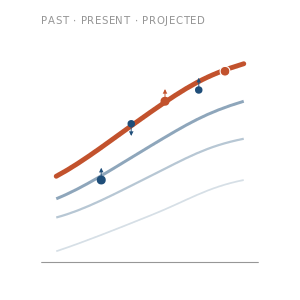
\includegraphics[height=6mm]{yc_logo.png}}
  \hfill{\ttfamily\scriptsize\color{ycmuted}yieldcartography.com/slides/eh/}
\end{frame}

\end{document}
